\section{Differenzstufe: Differenzaussteuerung}
In diesem Versuchsteil soll die Differenzstufe mit einem differentiellen Eingangssignal
ausgesteuert werden.
F\"ur diesen Versuchsteil wird ein differentielles AC-Eingangssignal ben\"otigt. Dieses
wird mit einem Symmetrie\"ubertrager generiert. An dessen Eingang wird der
Funktionsgenerators angeschlossen. Am Ausgang erh\"alt man ein differentielles
Ausgangssignal, welches ungef\"ahr um den Faktor 10 kleiner ist als das
Eingangssignal.
\subsection{Experimentelle Durchf\"urung}
Die Schaltung aus Versuch 2 wurde mit einem 2~$k \Omega$ Potentiometer erg
\"anzt. Dieser wurde so eingestellt, dass sich U$_{aus}$~$=$~0V ergab, wobei 
$_{ein,p}$ und U$_{ein,n}$~$=$~0V betragen muss. Mit dieser Einstellung wurde 
der Arbeitspunkt erneut vermessen. Anschlie\ss end wurde der differentielle 
Eingangsspannungsbereich vermessen, daf\"ur wurde eine differentielle DC 
Spannung um 0V herum angelegt. Als n\"achstes wurde ein Symmetrie\"ubertr
\"ager verwendet, dieser wurde mit einem differentiellen AC-Signal mit 
Frequenz von 1~$kHz$ und einer Signalamplitude von 500~$mV$ verbunden. Mit 
diesem Aufbau wurde die Amplitude des differentiellen Eingangs- und 
Ausgangssignal bestimmt. Zum Schluss wurde die beiden Eing\"ange U$_{ein,p}~$=U
$_{ein,n} $ = U$_{ein}$ kurzgeschlossen und wiederum die Amplituden bestimmt.
\begin{figure}[!ht]
\begin{center}
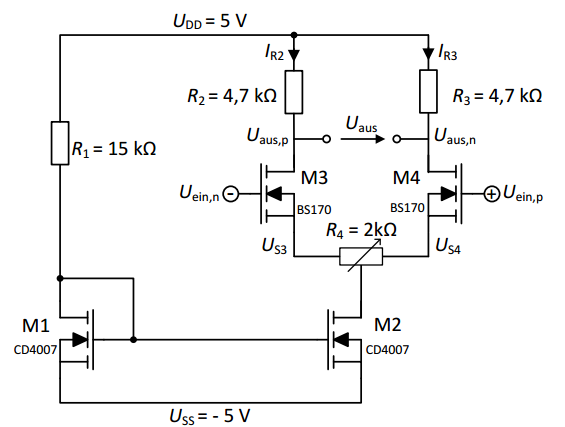
\includegraphics[scale=0.8]{Differenzstufe1}
\end{center}
\end{figure}
\subsection{Ergebnisse und Diskussion}
\begin{figure}[!ht]
\begin{center}

\includegraphics[scale=0.8]{Text}
\end{center}
\end{figure}
\begin{figure}[!ht]
\begin{center}
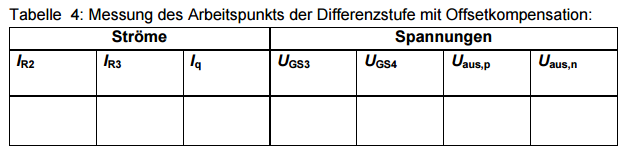
\includegraphics[scale=0.8]{Tabelle4}
\end{center}
\end{figure}
\begin{figure}[!ht]
\begin{center}
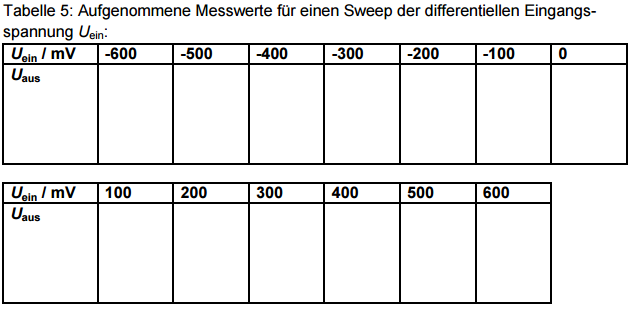
\includegraphics[scale=0.8]{Tabelle5}
\end{center}
\end{figure}
\begin{figure}[!ht]
\begin{center}

\includegraphics[scale=0.8]{Text}
\end{center}
\end{figure}
\begin{figure}[!ht]
\begin{center}
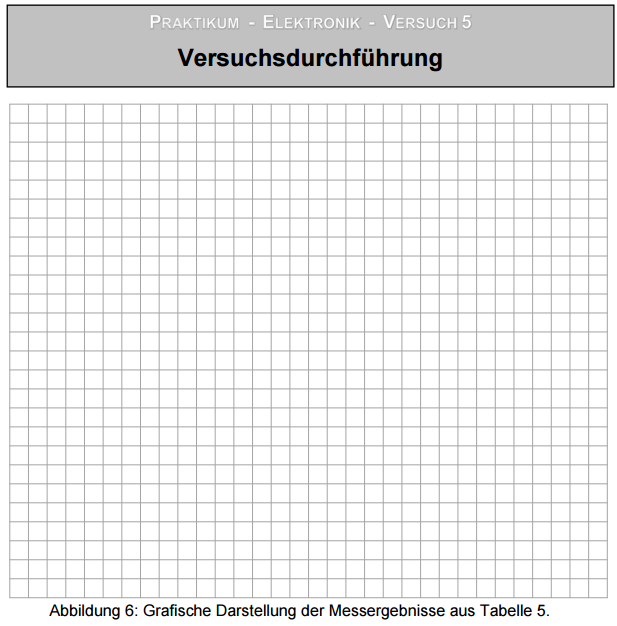
\includegraphics[scale=0.8]{Graph3}
\end{center}
\end{figure}
\newpage
\begin{figure}[!ht]
\begin{center}
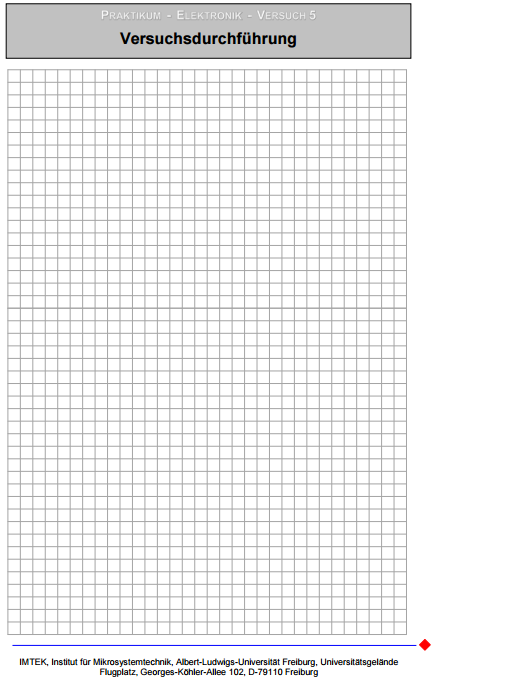
\includegraphics[width = 1.3\textwidth]{Write}
\end{center}
\end{figure}
\newpage
\begin{figure}[!ht]
\begin{center}
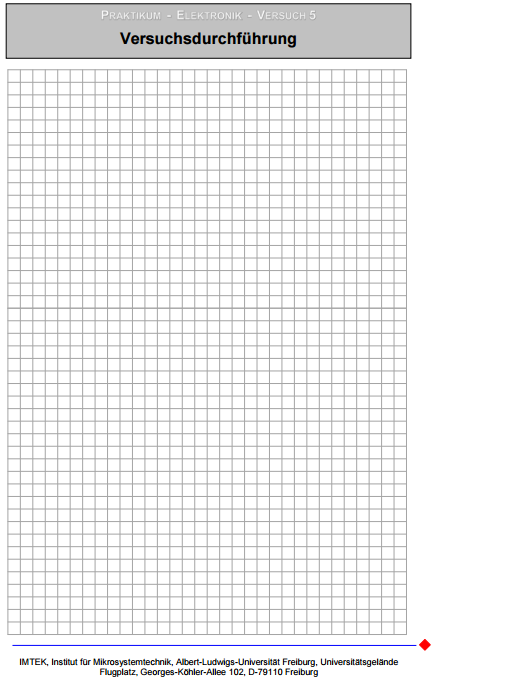
\includegraphics[width = 1.3\textwidth]{Write}
\end{center}
\end{figure}
\newpage
\begin{figure}[!ht]
\begin{center}
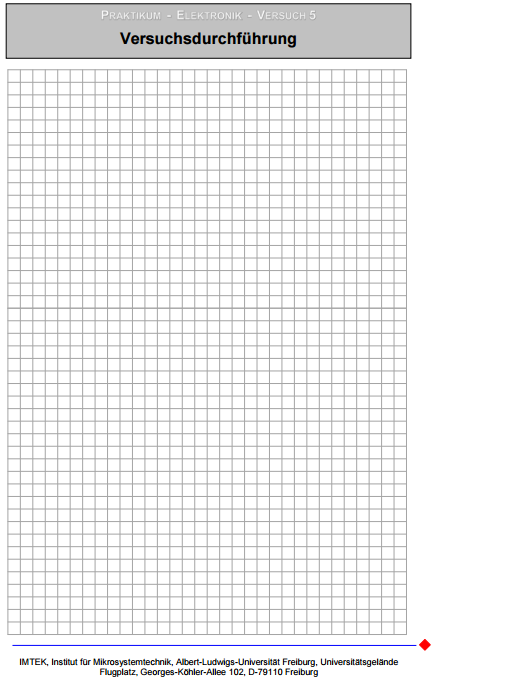
\includegraphics[width = 1.3\textwidth]{Write}
\end{center}
\end{figure}
\newpage
\begin{figure}[!ht]
\begin{center}
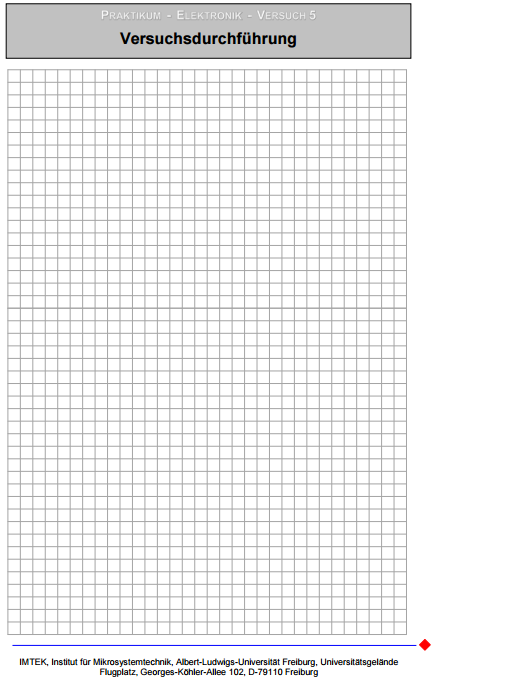
\includegraphics[width = 1.3\textwidth]{Write}
\end{center}
\end{figure}
\newpage
\begin{figure}[!ht]
\begin{center}
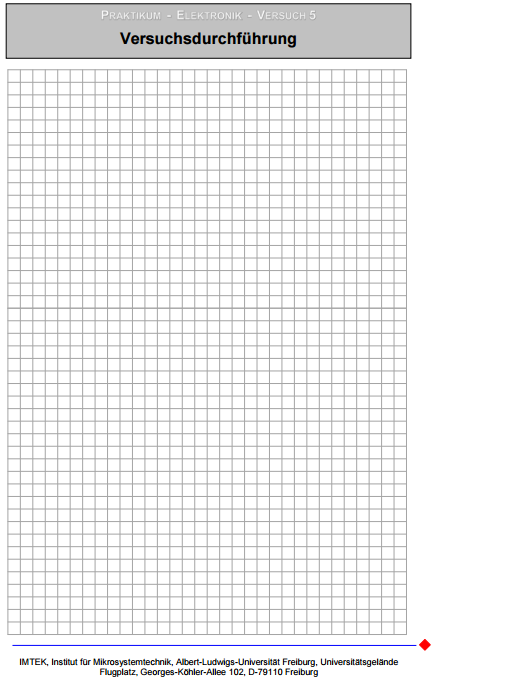
\includegraphics[width = 1.3\textwidth]{Write}
\end{center}
\end{figure}